\documentclass[tikz, border=0]{standalone}
\usepackage{fontspec}
\usepackage{unicode-math}
\usetikzlibrary{shapes.geometric}

\setmainfont{TeX Gyre Pagella}
\setmathfont{TeX Gyre Pagella Math}
\usetikzlibrary{calc,arrows.meta,patterns, shapes.geometric, calc, backgrounds}

\definecolor{Red}{HTML}{9f2430}
\definecolor{LBlue}{RGB}{ 186, 220, 255 }
\definecolor{DBlue}{HTML}{132C53} 
\definecolor{gray}{HTML}{708090}
\definecolor{LGreen}{RGB}{185, 230, 200}
\definecolor{LRed}{HTML}{f97ffd}

\NewDocumentCommand{\DrawPolyadic}{O{0} O{7} O{Polyadic}}{
    
    \begin{scope}[shift={(#1,0)}]
        \node[anchor=south, regular polygon, regular polygon sides=#2, minimum size=10em, fill=LBlue] (poly) at (0,0) {};
        \foreach \i in {1,...,#2} {
            \draw[line width=0.08em, white, fill=DBlue] (poly.corner \i) circle (0.5em);
        }
        \node[white, font=\bfseries] at (0,-2em) {#3};
    \end{scope}
}

\NewDocumentCommand{\DrawSimplicialComplex}{O{0} O{7} O{S. Complex}}{
    
    \begin{scope}[shift={(#1,0)}]
        \node[anchor=south, regular polygon, regular polygon sides=#2, minimum size=10em] (poly) at (0,0) {};
        \foreach \i in {1,...,#2} {
        \foreach \j in {\i,...,#2} {
            \draw[Red, ultra thick] (poly.corner \j) -- (poly.corner \i);
        }
            \draw[line width=0.08em, white, fill=DBlue] (poly.corner \i) circle (0.5em);
        }
        \node[white, font=\bfseries] at (0,-2em) {#3};
    \end{scope}
}

\NewDocumentCommand{\DrawPair}{O{0} O{Polygon} O{Red}}{
    
    \begin{scope}[shift={(#1,0)}]
        \coordinate (top) at (0,7);
        \coordinate (bottom) at (0,0);
        \draw[draw=none] (-5,0) -- (5,0);
        \draw[#3, ultra thick] (top) -- (bottom);
        \draw[line width=0.08em, white, fill=DBlue] (top) circle (0.5em);
        \draw[line width=0.08em, white, fill=DBlue] (bottom) circle (0.5em);
        \node[white, font=\bfseries] at (0,-2em) {#2};
    \end{scope}
}

\begin{document}

\begin{tikzpicture}[x=1em, y=1em]

    \useasboundingbox (-31,-17) rectangle (31,17);

    \begin{scope}[shift={(0,5)}]
        \node[white,  font=\large\bfseries] at (0,10em) {Higher-order interactions};
        \DrawPair[-24][Dyadic interaction][LBlue]
        \DrawPolyadic[-12][3][Triadic interaction]
        \DrawPolyadic[0][4][Tetradic interaction]
        \DrawPolyadic[12][5][Pentadic interaction]
        \DrawPolyadic[24][6][Hexadic interaction]
    \end{scope}
\end{tikzpicture}

\begin{tikzpicture}[x=1em, y=1em]

    \useasboundingbox (-31,-17) rectangle (31,17);

    \begin{scope}[shift={(0,-13)}]
        \node[white,  font=\large\bfseries] at (0,10em) {All-to-all pair approximation};
        \DrawPair[-24][$K_2$]
        \DrawSimplicialComplex[-12][3][$K_3$]
        \DrawSimplicialComplex[0][4][$K_4$]
        \DrawSimplicialComplex[12][5][$K_5$]
        \DrawSimplicialComplex[24][6][$K_6$]
    \end{scope}
\end{tikzpicture}

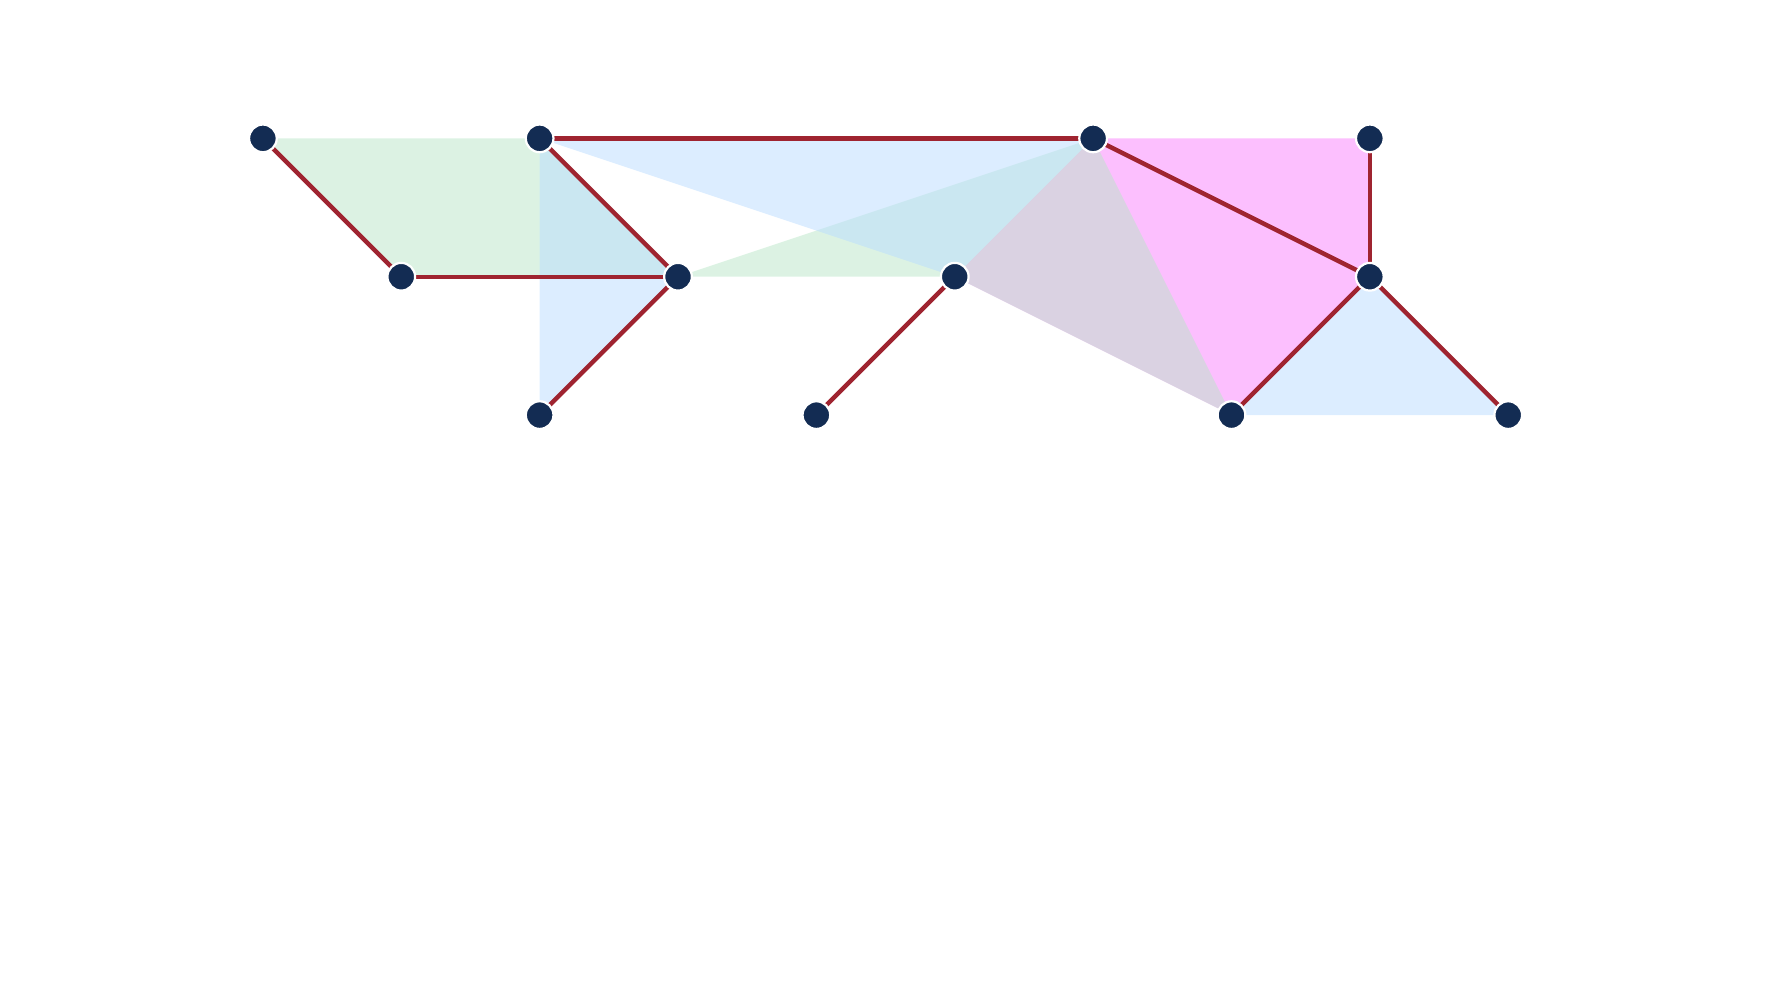
\begin{tikzpicture}[x=1em, y=1em]

    \def\N{15}
    \def\Ylim{5}
    \def\Xlim{5}

    \useasboundingbox (-31,-17) rectangle (31,17);

    \begin{scope}[shift={(0,3)}]
        \node[white,  font=\large\bfseries] at (0,12em) {Higher-order network};
        \begin{scope}[shift={(-4.5*\Xlim,\Ylim)}, name prefix=node-]
            \coordinate (1) at (0,\Ylim);
            \coordinate (2) at (\Xlim,0);
            \coordinate (3) at (2*\Xlim,\Ylim);
            \coordinate (4) at (2*\Xlim,-\Ylim);
            \coordinate (5) at (3*\Xlim,0);
            \coordinate (6) at (4*\Xlim,-\Ylim);
            \coordinate (7) at (5*\Xlim,0);
            \coordinate (8) at (6*\Xlim,\Ylim);
            \coordinate (9) at (7*\Xlim,-\Ylim);
            \coordinate (10) at (8*\Xlim,\Ylim);
            \coordinate (11) at (8*\Xlim,0);
            \coordinate (12) at (9*\Xlim,-\Ylim);
        \end{scope}
        
        % 5
        \fill[LRed, opacity=0.5]
            (node-10) -- (node-8) -- (node-7) -- (node-9) -- (node-11) -- cycle;

        % Tetradics
        \fill[LGreen, opacity=0.5]
            (node-1) -- (node-2) -- (node-5) -- (node-3) -- cycle;
        \fill[LGreen, opacity=0.5]
            (node-5) -- (node-7) -- (node-9) -- (node-8) -- cycle;

        % Triadics
        \fill[LBlue, opacity=0.5]
            (node-11) -- (node-9) -- (node-12) -- cycle;
        \fill[LBlue, opacity=0.5]
            (node-3) -- (node-4) -- (node-5) -- cycle;
        \fill[LBlue, opacity=0.5]
            (node-3) -- (node-7) -- (node-8) -- cycle;

        % Dyadics
        \draw[Red, ultra thick] (node-1) -- (node-2);
        \draw[Red, ultra thick] (node-2) -- (node-5);
        \draw[Red, ultra thick] (node-3) -- (node-5);
        \draw[Red, ultra thick] (node-3) -- (node-8);
        \draw[Red, ultra thick] (node-4) -- (node-5);
        \draw[Red, ultra thick] (node-6) -- (node-7);
        \draw[Red, ultra thick] (node-8) -- (node-11);
        \draw[Red, ultra thick] (node-9) -- (node-11);
        \draw[Red, ultra thick] (node-10) -- (node-11);
        \draw[Red, ultra thick] (node-11) -- (node-12);

        \foreach \i in {1,...,12} {
            \draw[line width=0.08em, white, fill=DBlue] (node-\i) circle (0.5em);
        }
    \end{scope}
    
\end{tikzpicture}

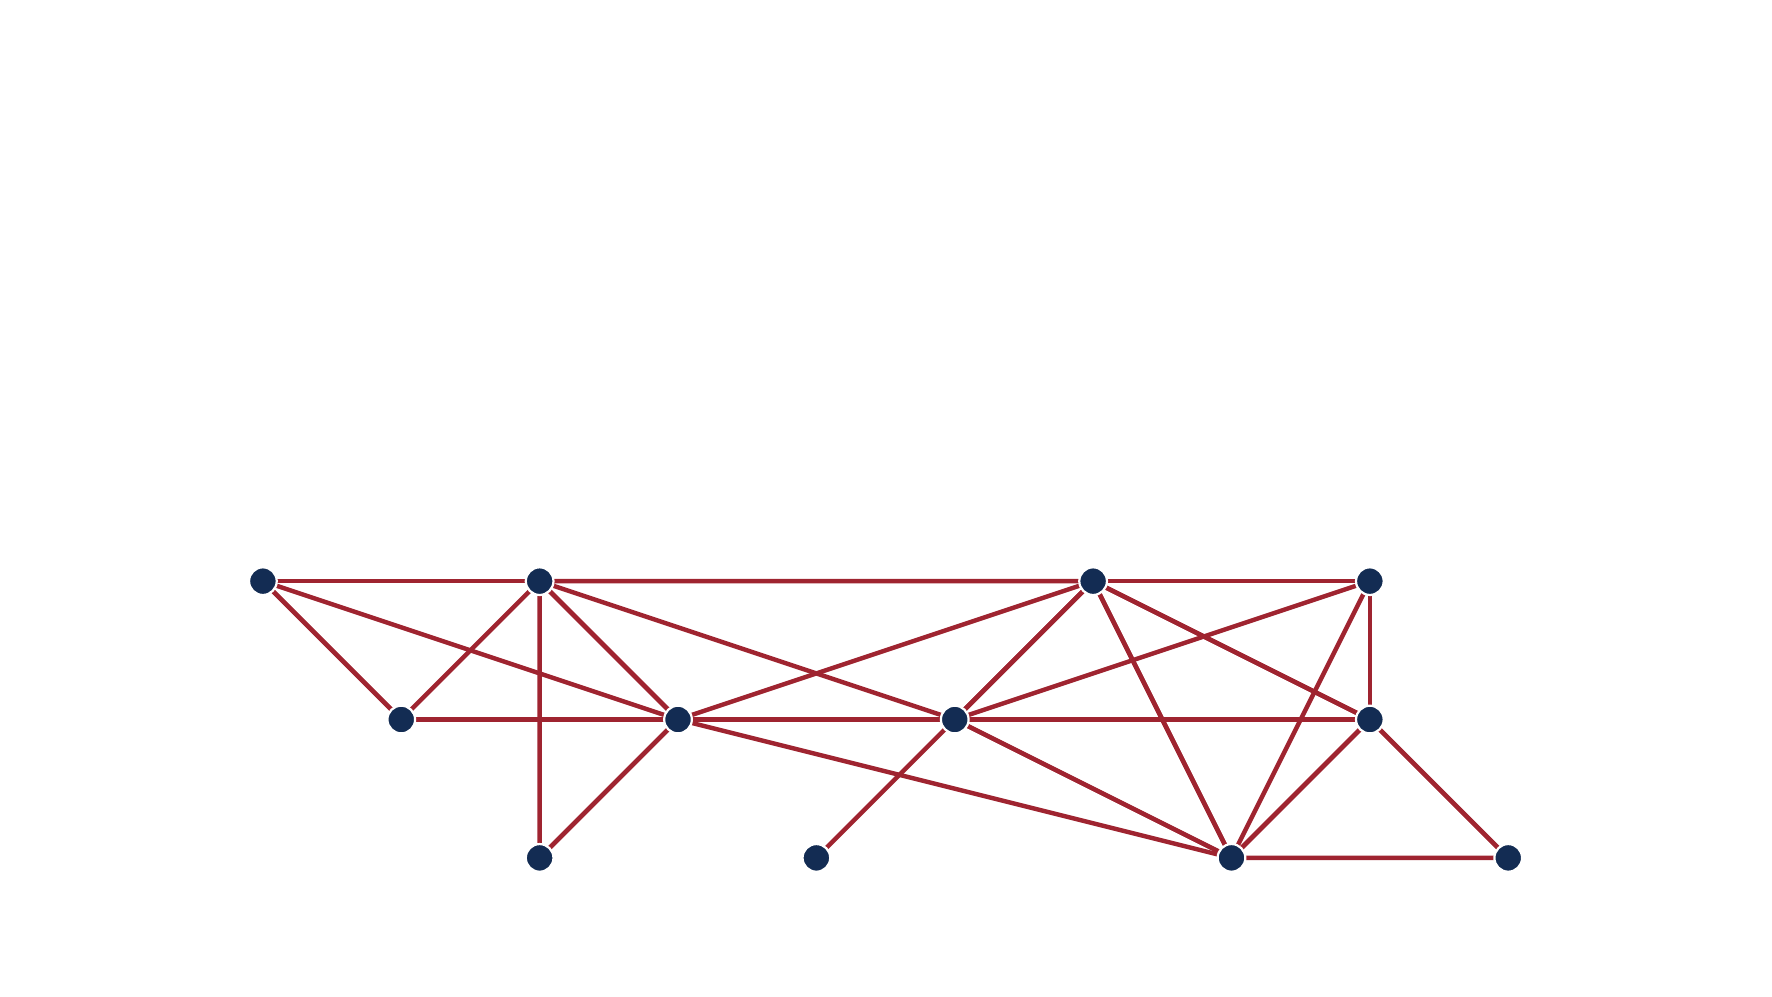
\begin{tikzpicture}[x=1em, y=1em]

    \def\N{15}
    \def\Ylim{5}
    \def\Xlim{5}

    \useasboundingbox (-31,-17) rectangle (31,17);

    \begin{scope}[shift={(0,-13)}]
        \node[white,  font=\large\bfseries] at (0,12em) {All-to-all pair approximation};
        \begin{scope}[shift={(-4.5*\Xlim,\Ylim)}, name prefix=node-]
            \coordinate (1) at (0,\Ylim);
            \coordinate (2) at (\Xlim,0);
            \coordinate (3) at (2*\Xlim,\Ylim);
            \coordinate (4) at (2*\Xlim,-\Ylim);
            \coordinate (5) at (3*\Xlim,0);
            \coordinate (6) at (4*\Xlim,-\Ylim);
            \coordinate (7) at (5*\Xlim,0);
            \coordinate (8) at (6*\Xlim,\Ylim);
            \coordinate (9) at (7*\Xlim,-\Ylim);
            \coordinate (10) at (8*\Xlim,\Ylim);
            \coordinate (11) at (8*\Xlim,0);
            \coordinate (12) at (9*\Xlim,-\Ylim);
        \end{scope}

        % Dyadics
        \draw[Red, ultra thick] (node-1) -- (node-2);
        \draw[Red, ultra thick] (node-2) -- (node-5);
        \draw[Red, ultra thick] (node-3) -- (node-5);
        \draw[Red, ultra thick] (node-3) -- (node-8);
        \draw[Red, ultra thick] (node-4) -- (node-5);
        \draw[Red, ultra thick] (node-6) -- (node-7);
        \draw[Red, ultra thick] (node-8) -- (node-11);
        \draw[Red, ultra thick] (node-9) -- (node-11);
        \draw[Red, ultra thick] (node-10) -- (node-11);
        \draw[Red, ultra thick] (node-11) -- (node-12);
                
        
        % Triadics
        \draw[Red, ultra thick]
            (node-11) -- (node-9) -- (node-12) -- cycle;
        \draw[Red, ultra thick]
            (node-3) -- (node-4) -- (node-5) -- cycle;
        \draw[Red, ultra thick]
            (node-3) -- (node-7) -- (node-8) -- cycle;

        % Tetradics
        \foreach \i in {1,2,5,3} {
            \foreach \j in {1,2,5,3} {
                \ifnum \i<\j
                    \draw[Red, ultra thick] (node-\i) -- (node-\j);
                \fi
            }
        }
        \foreach \i in {5,7,8,9} {
            \foreach \j in {5,7,8,9} {
                \ifnum \i<\j
                    \draw[Red, ultra thick] (node-\i) -- (node-\j);
                \fi
            }
        }

        % 5
        \foreach \i in {7,8,9,10,11} {
            \foreach \j in {7,8,9,10,11} {
                \ifnum \i<\j
                    \draw[Red, ultra thick] (node-\i) -- (node-\j);
                \fi
            }
        }

        \foreach \i in {1,...,12} {
            \draw[line width=0.08em, white, fill=DBlue] (node-\i) circle (0.5em);
        }
    \end{scope}
    
\end{tikzpicture}


\end{document}

